\chapter{Application -- Theoretical Background and Practical Implementation}
%\section{Theoretical background}

\section{Geometric Brownian Motion}\index{Geometric Brownian Motion}
    This section focuses on explaining what \textit{Geometrical Brownian Motion} is and how it can be implemented in the F\# language.
    
    \subsection{Geometric Brownian Motion -- Introduction}
        \textit{Geometric Brownian Motion} is often used as a model for simulating diverse variables. Therefore, financial processes, such as stock prices, are frequently modeled using \textit{GBM}. In order to define correctly what a \textit{GBM} is, it is essential to first describe several terms that will help further understanding.
    
    \subsection{Random Walk}\index{Random Walk}
        \textit{Random Walk} is a stochastic process used in mathematics that illustrates how objects might travel if they were to move randomly, more details here \cite{randomWalk}.
        %
        If 1D space is taken into account, then it is best to present the action on the number line.
        \begin{figure}[H]
            \centering
            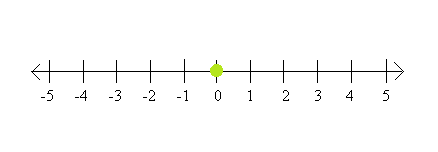
\includegraphics{img/numberLine.png}
            \caption{Number line with starting point $P_0=0$}
            \caption*{$P$ stands for \textit{Position}.}
            \label{fig:numberLine_start}
        \end{figure}
        %
        Random walk starts at the point 0 (fig. \ref{fig:numberLine_start}). Then there occur $N$ steps, $N \in \mathbb{N}_+$, and each of them is likely to move to the right ($+1$) or to the left ($-1$) by 50\%. The exemplary outcome after 4 steps could be as follows:
        %
        \begin{figure}[H]
            \centering
            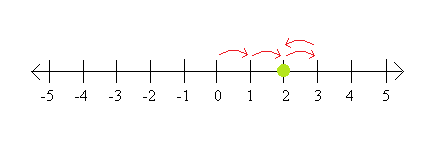
\includegraphics{img/numberLine_end.png}
            \caption{Sample outcome for $N=4$.}
            \label{fig:numberLine_end}
        \end{figure}
        %
        In this example the steps could be described as $a_1 = a_2 = a_3 = 1$ and $a_4 = -1$, meaning the first 3 steps were to the right, while the last one was to the left. The outcome (position of the green dot after all the steps) is $P_4 = 2$ (fig. \ref{fig:numberLine_end}).
        %
        Therefore, the position of the green dot can be specified by the following formula:
        \[  % \ldots looks better than ...
        P_N = a_1 + a_2 + a_3 + \ldots + a_N
        .
        \]
        %
        \textit{Random Walk} $RW$ can then defined as the following series:
        \[
        RW = \{P_n, n \in N\}
        .
        \]
        %
        Since each move has the same probability (can be either $-1$ or $+1$) then the expected value of such series (the final position of the dot) can be easily calculated as follows:
        \[
        \mathbb{E}(RW) = 0
        .
        \]
        
        An interesting observation can be made when calculating an estimated value of a series that is the same as \textit{Random Walk} but its values are squares of the original values.
        % I should use \(...\) instead of $...$
        Then:
        \[
        \mathbb{E}({RW}^2) = \sum_{i=1}^{N} a_{i} + 2*\sum_{1 \leq i \leq j \leq N}^{N} a_{i}*a_{j} = N
        .
        \]
        %
        Therefore, the average distance that the dot will appear on at the end of the walk will be at \(\sqrt{N}\) blocks from the starting position.
        
    \subsection{Wiener Process}\index{Wiener Process}
        The \textit{Wiener Process} is also usually called the \textit{Standard Brownian Motion}. It is a continuous-time stochastic process named after Norbert Wiener for his work on 1D \textit{Brownian Motion}.
        %
        \textit{Wiener Process}, as well as \textit{Random Walk}, starts at 0 (\( W(0) = 0 \)) and its increment follows Gaussian distribution with mean \(0\) and variance \(t-s\) for any \(0\leq s < t \) (more details here \cite{wienerProcess}).
        %
        This way a \textit{Brownian Motion} is basically a \textit{Random Walk} with steps which sizes are random.
    \subsection{Geometric Brownian Motion -- Explanation}
        Finally, having \textit{Standard Brownian Motion} covered, it is the right time to explain what the Geometric version is. One of the biggest disadvantages of the Wiener Process is the fact that it can reach negative values. When treated as a tool for simulating stock prices, such a flaw is disqualifying. Otherwise, it might lead to a situation, where certain stock's price goes below zero which would mean that one might actually get paid in order to obtain shares in the ownership of some corporation. Such a scenario never happens in reality, in contrast to interest rates (more information about negative interest rates can be found here: \cite{negativeInterestRates}).
        
        \textit{Geometric Brownian Motion} is a stochastic process, also called \textit{Exponential Brownian Motion} due to the exponent occurring in its formula:
        \[
        S_t = S_0e^{(\mu - \frac{\sigma^2}{2})t + \sigma W_t}
        ,
        \]
        where:
        \begin{itemize}
        \item $S_t$ - underlying asset price at the moment $t$,
        \item $S_0$ - underlying asset price at the beginning ($t=0$),
        \item $\mu$ - drift (7\% represented as 0.07),
        \item $\sigma$ - volatility (20\% represented as 0.2),
        \item $W_t$ - Wiener process' (Standard Brownian Motion) value at the moment $t$.
    \end{itemize}
    %
    The key to understanding constant parameters $\mu$ -- drift and $\sigma$ -- volatility is to pair the former with modeling deterministic trends while the latter with the amount of unpredictable events occurrences during the motion (more information about \textit{GBM} can be found here \cite{gbm}).
    
    To create \textit{Geometric Brownian Motion}, \textit{Wiener Process} based on random normal variables is required. Since, in F\# language there is no default library containing such variables generator, one can use \textit{Box-Muller Transform}. For two independently uniformly distributed random variables $U_1$ and $U_2$ that come from a distribution on the interval $[0,1]$, \textit{Box-Muller Transform} creates 2 independent, \textbf{normal} random variables $N_1$ and $N_2$:
    \[
    N_1 = \sqrt{-2\ln{U_1}}\sin(2\pi U_2), N_2 = \sqrt{-2\ln{U_1}}\cos(2\pi U_2)
    .
    \]
    
    Undermentioned listing shows possible implementation of \textit{GBM}.
    \begin{lstlisting}[caption=F\# implementation of \textit{Geometric Brownian Motion}.]
//generates list of n Uniform RVs from interval [0,1]
let genRandomNumbersNominalInterval (count:int) (seed:int) : float list =
    let rnd = System.Random(seed)
    List.init count (fun _ -> rnd.NextDouble())

//input: UniformRM need to be from interval (0,1]
//input: steps must be even
//output: NormalRV have mean=0 and standard_deviation=1
let normalizeRec (uniformList:float list) (n:int) : float list =
    let rec buildNormalList (normalList:float list) =
        if normalList.Length = n then normalList
        else
            let currentNIdOne = normalList.Length
            let currentNIdTwo = currentNIdOne + 1
            let oneU = uniformList.[currentNIdOne]
            let twoU = uniformList.[currentNIdTwo]
            let oneN = sqrt(-2.*Math.Log(oneU, Math.E))*sin(2.*Math.PI*twoU)
            let twoN = sqrt(-2.*Math.Log(oneU, Math.E))*cos(2.*Math.PI*twoU)
            let newUniforms = [oneN; twoN]
            buildNormalList (normalList@newUniforms)
        buildNormalList []
let simulateGBM (count:int) (steps:int) (price:float) (drift:float) (vol:float) (years:float) (seed:int) =
    let normalRV = normalizeRec (genRandomNumbersNominalInterval steps seed) steps
    //build stock prices list
    let rec buildStockPricesList (currentStockPricesList:float list) (steps:int) (normalId:int) : float list =
        if normalId = steps-1 then currentStockPricesList
        else
            let firstExpTerm =  (drift - (vol**2.)/2.) * (float(years)/float(steps))
            let secondExpTerm =  vol * sqrt(float(years)/float(steps)) * normalRV.[normalId]
            let newStockPrice = currentStockPricesList.[normalId] * Math.E ** (firstExpTerm + secondExpTerm)
            buildStockPricesList (currentStockPricesList@[newStockPrice]) steps (normalId+1)
    let stockPricesList = buildStockPricesList [price] steps 0
    stockPricesList
        \end{lstlisting}
    %
    Figures \ref{fig:gbm_dri} and \ref{fig:gbm_vol} show how parameters such as the drift and the volatility affect trends generated by \textit{GBM}. While drift ($\mu$) is responsible for overall trend (whether stock prices rise overtime ($\mu$ > 0) or drop very rapidly ($\mu$ << 0)), volatility is a parameter describing dispersion of values. If it is high, then the dispersion is high as well (see red trend in the Fig. \ref{fig:gbm_vol}).
        \begin{figure}[H]
            \centering
            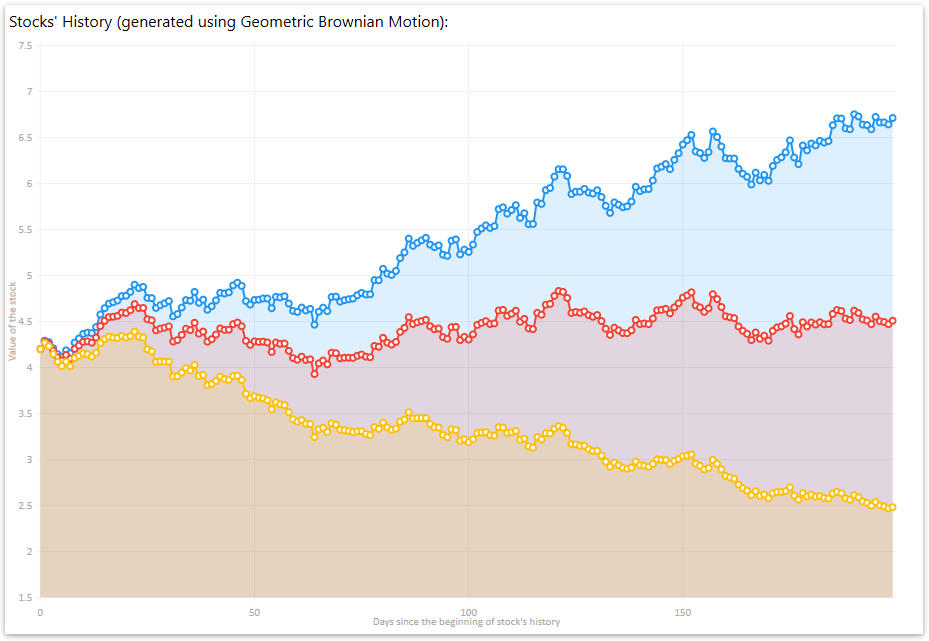
\includegraphics[width=\textwidth]{img/gbm_dri_06_02andm08.png}
            \caption{\textit{GBM} trends when drift ($\mu$ parameter) is changing:}
            \caption*{Source: \textit{MARS App}}
            \caption*{blue: $\mu = 0.6$,}
            \caption*{red: $\mu = 0.2$,}
            \caption*{yellow: $\mu = -0.8$.}
            \label{fig:gbm_dri}
        \end{figure}
        
        \begin{figure}[H]
            \centering
            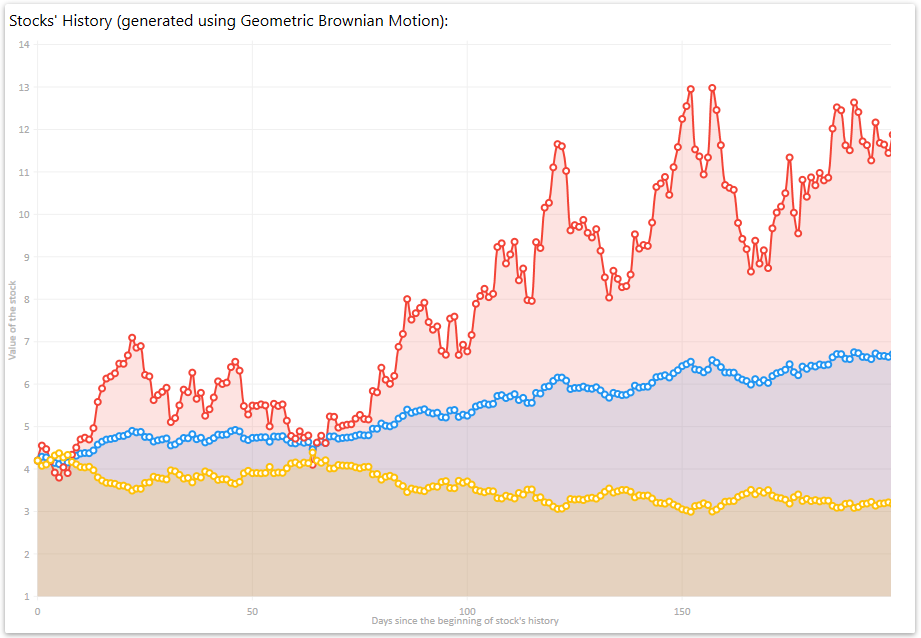
\includegraphics[width=\textwidth]{img/gbm_vol_08_02andm03.png}
            \caption{\textit{GBM} trends when volatility ($\sigma$ parameter) is changing:}
            \caption*{Source: \textit{MARS App}}
            \caption*{red: $\sigma = 0.8$,}
            \caption*{blue: $\sigma = 0.2$,}
            \caption*{yellow: $\sigma = -0.3$.}
            \label{fig:gbm_vol}
        \end{figure}
    
\section{Options}\index{Option}
    Options are some of the most popular derivative financial instruments. Derivative means in this example that it's value is reliant upon an underlying asset. The most important thing about options, one that distinguishes them from other derivative instruments it the \textbf{optionality} -- contract can, but is not obligatory to be made.
    
    There are 2 main types of options:
    \begin{itemize}
        \item \textbf{Call option}\index{Call Option} -- the buyer of such option buys himself a right (it is not an obligation) to exercise the option (buy an underlying asset) from the option seller after the option has reached its maturity.
        \item \textbf{Put option}\index{Put Option} -- the buyer of such option buys himself a right to sell an underlying asset to the option seller after the option has reached its maturity. 
    \end{itemize}
    \noindent
    More about the options definitions can be found here \cite{Call_Put_Option_Definition}.
    
    There are several parameters that describe an option, most important ones are:
    \begin{itemize}
        \item \textbf{Expiration Date} -- Specific moment in time by which the holder of the option has to decide whether he wants to exercise (use) the option.
        \item \textbf{Strike Price} -- agreed price at which the derivative underlying asset can be bought or sold (depends on a type of option) when it is exercised.
    \end{itemize}
    %
    \index{Expiry}
    \noindent
    Further division into option types depends on when the option can be exercised. The most basic one is a \textbf{European}-style option -- the decision whether option will or will not be exercised is made at the time of the option's expiry. A continuous option type is an \textbf{American}--style option -- option can be exercised at any time before the expiry. Combination of those two can be found in the \textbf{Burmudan}--style option -- the contract can be exercised at specific days before the expiration. In this paper European options will be presented (more about option types in \cite{Option_Types}).
    
    The code which implements options is as follows:
    \begin{lstlisting}[label={lst:option}, caption=F\# implementation of an option.]
type CallOrPutFlag =
    | Call
    | Put
    override this.ToString() =
               match this with
               | Call -> "Call"
               | Put -> "Put"
               
type OptionRecord =
    (* Model for Option Record. *)
    {
        OptionName:     string
        Expiry:         DateTime
        Strike:         float
        CallOrPutFlag:  CallOrPutFlag
        StockPrice:     float
        UnderlyingStock:Stock
    }

    (* Simple utility method for creating a random option. *)
    static member sysRandom = System.Random()
    static member Random (calc : CalculationParameters) (market : MarketData) =
        let rnd  = System.Random()
        (* Below OptionRecord type  will be returned *)
        {
            OptionName      = sprintf "Option%03d" (OptionRecord.sysRandom.Next(999))
            Expiry          = (DateTime.Now.AddMonths(OptionRecord.sysRandom.Next(2, 12))).Date
            Strike          =
                let s =
                    match market.TryFind "stock::price" with
                    | Some price -> float price
                    | None -> 6.70  // default 6.70$ for stock price
                s*1.1   //Strike price is 110% of stock price
            
            CallOrPutFlag   = 
                if rnd.Next()%2 |> System.Convert.ToBoolean then
                    Call
                else
                    Put
            
            StockPrice      =
                let s =
                    match market.TryFind "stock::price" with
                    | Some price -> float price
                    | None -> 6.70  // default 6.70$ for stock price
                s
            UnderlyingStock = Stock.Random (calc: CalculationParameters) (market : MarketData)
        }
    \end{lstlisting}
    
    \noindent
    Generating options is presented in Figure \ref{fig:optionsPresentation}:
    \begin{figure}[H]
            \centering
            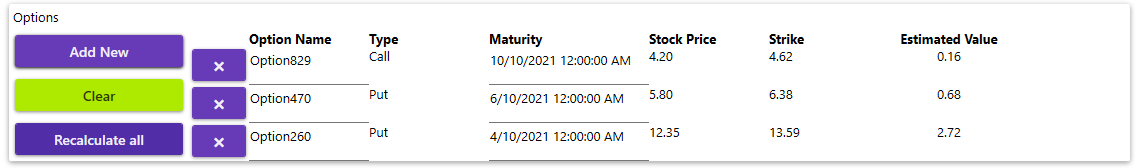
\includegraphics[width=\textwidth]{img/optionsPresentation.png}
            \caption{Options view in the application.}
            \caption*{Source: \textit{MARS App}}
            \label{fig:optionsPresentation}
    \end{figure}
    
    \noindent
    Before an option is generated, the user is able to specify parameters affecting the calculation, as shown in Fig. \ref{fig:parametersPresentation}.
    \begin{figure}[H]
            \centering
            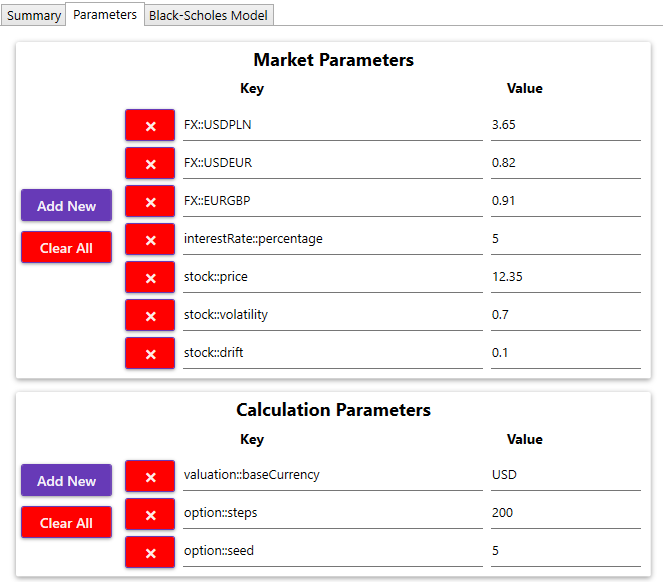
\includegraphics[width=\textwidth]{img/specifyParameters.png}
            \caption{Parameters specification for options generation and valuation.}
            \caption*{Source: \textit{MARS App}}
            \label{fig:parametersPresentation}
    \end{figure}
\section{Black-Scholes Model}\index{Black-Scholes Model} \index{Fisher Black} \index{Myron Scholes} \index{Robert Merton}
    The Black--Scholes formula was created back in 1970s by 3 great economists: Fischer Black, Myron Scholes and Robert Merton (Scholes and Merton were later awarded Nobel Prize in Economics in 1997. We may assume same would happen for Black if sadly it was not for his death in 1975). That why this model is sometimes also called Black--Scholes--Merton.
    %
    Their model was a significant breakthrough in the world of mathematical models used for pricing derivative instruments. It provides a framework for European-style option valuations, such as calls and puts.
    
    This thesis' aim was not to goo too deep into the understanding of the mathematical background behind the model but rather to implement the model in a practical tool that one would be able to effectively use. Therefore more information and specifics can be found in the original publication \cite{10.2307/1831029} of the model from 1973 in \textit{The Pricing of Options and Corporate Liabilities} of the Journal of Political Economy by Fischer Black and Myron Scholes.
    
    The main formula of the model used for option pricing is as follows:
    \[
    C = S_0\phi(d_1) - Ke^{-rt}\phi(d_2)
    ,
    \]
    \[
    P = -S_0\phi(-d_1) + Ke^{-rt}\phi(-d_2)
    ,
    \]
    \[
    d_1 = ln\frac{S_0}{K} + (r+\frac{\sigma^2}{2})t
    ,
    \]
    \[
    d_2 = d_1 - \sigma\sqrt{t}
    ,
    \]
    where:
    \begin{itemize}
        \item $C$ - call option price,
        \item $P$ - put option price,
        \item $S_0$ - current price of an underlying asset,
        \item $\phi()$ - standardized cumulative normal distribution,
        \item $K$ - strike price,
        \item $r$ - risk free rate (1\% represented as 0.01),
        \item $t$ - time to maturity in years (18 months represented as 1.5),
        \item $\sigma$ - volatility (20\% represented as 0.2).
    \end{itemize}
    %
    The formula assumes that the price history of an underlying asset (in this example - a stock price) has a lognormal distribution and follows \textit{Geometric Brownian Motion} with constant drift and volatility. \index{Drift}\index{Volatility}
    % \todo{diff eq thats at the core of the model as curiosity}
    %
    A simple analytical formula allows the model to be written in several lines of code thanks to the functional paradigm of the F\# language.
    \begin{lstlisting}[label={lst:bsm}, caption=F\# implementation of \textit{Black--Scholes Model}.]
    (* Black-Scholes for Option Valuation
    Parameters:
        call_or_put_flag (CallOrPutFlag):
            Flag that determines whether this option is put or call
        s0 (float): current price of an underlying asset (stock)
        k (float): strike price
        t (float): expiry date (counted in years from now on, e.g. 1.5)
        r (float): risk free rate (e.g. 0.05 means 5%)
        v (float): volatility (e.g. 0.2 means 20%)
    *)
    member this.BlackScholes() : float =
        let d1 = ( log(s0/k) + (r+v*v/2.)*t) / (v*sqrt(t))
        let d2 = d1 - v*sqrt(t)
        match call_or_put_flag with
        | Call -> s0*fi(d1) - k*exp(-r*t)*fi(d2)
        | Put ->  k*exp(-r*t)*fi(-d2) - s0*fi(-d1)
    \end{lstlisting}